\section{Problemy}

\subsection{Funkcja Rastrigina}

Pierwszym środowiskiem testowym jest funkcja Rastrigina, będąca abstrakcyjną funkcją testową. Charakteryzuje się ona tym, że posiada wiele minimów lokalnych oraz płaskie obszary, utrudniające odnalezienie minimum globalnego, przy użyciu gradientów.

\begin{figure}[H]
	\centering
	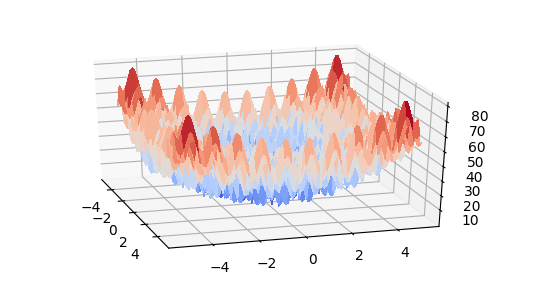
\includegraphics[width=\linewidth]{imgs/rastrigin_plot}
	\caption{Funkcja testowa.}
	\label{fig:rastrigin_plot}
\end{figure}

W implementacji wykorzystano funkcję Rastrigina zadaną wzorem:

$$f(x) = 10d + \sum_{i=1}^{d} [x_{i}^{2} - 10 \cos(2 \pi x_{i})]$$

gdzie $x_{i}$ oznacza wymiar, natomiast $d$ -- ich liczbę. Każde $x_{i}$ należy do przedziału $[-5.12; 5.12]$. 

\begin{figure}[H]
	\centering
	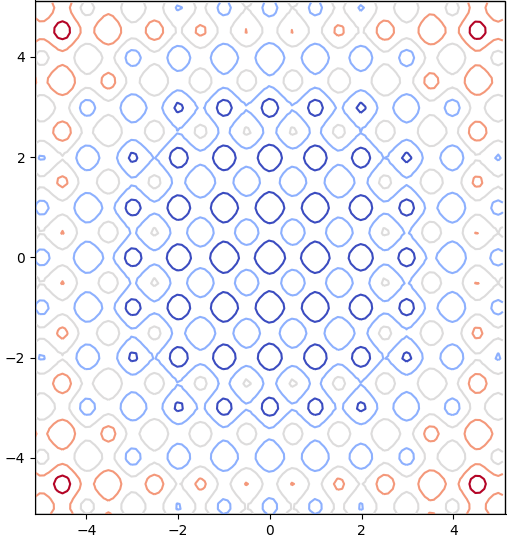
\includegraphics[width=0.4\linewidth]{imgs/rastrigin_2d_plot}
	\caption{Widok 2D funkcji testowej.}
	\label{fig:rastrigin_2d_plot}
\end{figure}


Przy badaniach poszukiwano minimum globalnego funkcji dwuwymiarowej. Rozwiązanie optymalne $f(x^{*})$, w uogólnieniu znajduje się w punkcie $x^{*} = (0, ..., 0)$. W problemie dwóch zmiennych znajduje się ono w punkcie $x^{*} = (0, 0)$.

\subsection{Funkcja Rastrigina z ograniczeniami}

Funkcja z ograniczeniami została zdefiniowana jak powyżej, jedną różnicą jest ograniczenie zakresu poszukiwań na każdej z osi $x_{i}$. W badaniach użyto zakresu $x_{i} = [-3; 3]$.

\begin{figure}[H]
	\centering
	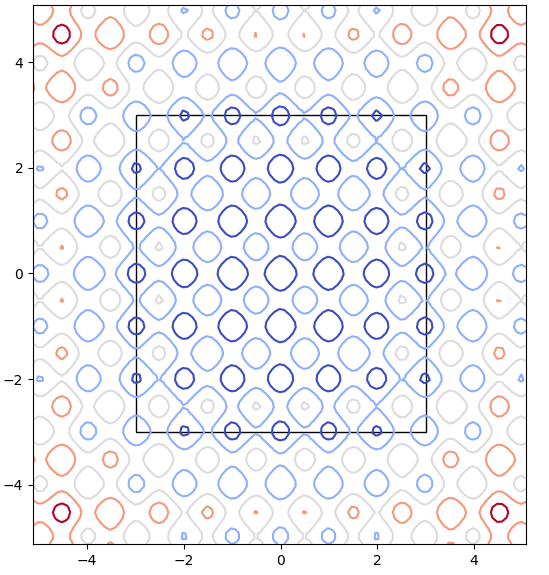
\includegraphics[width=0.4\linewidth]{imgs/rastrigin_2d_limited_plot}
	\caption{Widok 2D funkcji testowej z ograniczeniami.}
	\label{fig:rastrigin_2d_limited_plot}
\end{figure}

\pagebreak

\subsection{Projektowanie pokoju}

W problemie projektowania pokoju poszukiwano maksimum globalnego problemu. Zdefiniowane zostało ono jako maksymalizacja dywanu, którego centrum znajdowało się na środku pokoju (punkt $c_{c} = (0, 0)$). Podczas kolejnych iteracji starano się uzyskać jak największy promień $c_{r}$ dywanu, który przekładał się na jego większą powierzchnię. 

Przedmioty użyte w problemie:
\begin{table}[H]
	\centering
	\begin{tabular}{|c|c|c|c|c|}
		\hline
		\textbf{Przedmiot} & \textbf{Liczba} & \textbf{Szerokość} & \textbf{Wysokość} & \textbf{Umieszczenie na dywanie} \\
		\hline
		Szafa & 2 & 5 & 10 & Nie \\
		\hline
		TV & 1 & 5 & 2 & Nie \\
		\hline
		Sofa & 1 & 15 & 4 & Tak \\
		\hline
		Stół & 1 & 10 & 10 & Tak \\
		\hline
		Krzesło & 4 & 2.5 & 2.5 & Tak \\
		\hline
		Biurko & 1 & 7 & 13 & Nie \\
		\hline
		Okno & 1 & 2 & 10 & Tak \\
		\hline
		Drzwi & 1 & 8 & 4 & Tak \\
		\hline
	\end{tabular}
	\caption{Przedmioty użyte do modelowania pokoju.}
\end{table}

Ograniczenia wprowadzone do problemu:
\begin{itemize}
	\item nie wszystkie meble mogły zostać ustawione na dywanie -- z tego powodu, należało znaleźć odpowiednie ułożenie mebli, tak aby nie kolidowały one z dywanem;
	\item oprócz mebli, w pokoju znajdowały się również drzwi i okno. Nie mogły one zostać zasłonięte przez meble, których pozycje były zmieniane;
	\item kąt pomiędzy sofą a telewizorem nie mógł być większy niż \ang{30};
	\item odległość krzeseł od stołu powinna być minimalizowana.
\end{itemize}

Funkcja oceniająca dane rozwiązanie \emph{evaluate\_room}, jako argument przyjmowała aktualny stan pokoju. Kod tej funkcji prezentuje się następująco:

\begin{figure}[H]
	\begin{minted}{python}
def evaluate_room(room, intersections_weight=0.3, chairs_table_weight=0.1, tv_sofa_weight=0.1,
		inside_room_weight=0.4, carpet_weight=0.1):
		
	"""Should take an Room object and calculate the fitness (real number).
	Bigger value = better value."""
	
	total_reward = 0.0
	total_reward += intersections_weight * reward_for_intersections(room)
	total_reward += chairs_table_weight * reward_for_chairs_placement(room)
	total_reward += tv_sofa_weight * reward_for_tv_sofa_angle(room)
	total_reward += inside_room_weight * reward_for_furniture_inside_room(room)
	total_reward += carpet_weight * reward_for_carpet_size(room)
	
	return total_reward	
	\end{minted}
	\caption{Kod funkcji oceniającej finalny stan pokoju.}
\end{figure}

Kolejne funkcje zwracają następujące wartości:

\begin{itemize}
	\item \emph{\textbf{reward\_for\_intersections}(room)}: obszar, na którym nachodzą się dwa przemioty (meble, drzwi oraz okno) -- sprawdzane dla każdej pary;
	\item \emph{\textbf{reward\_for\_chairs\_placement}(room)}: zwracana jest odległość, w jakiej każde z krzeseł znajduje się od stołu;
	\item \emph{\textbf{reward\_for\_tv\_sofa\_angle}(room)}: jeśli kąt przekroczy \ang{30}, to zwracana jest wartość aktualnego kąta pomiędzy sofą a telewizorem;
	\item \emph{\textbf{reward\_for\_furniture\_inside\_room}(room)}: obszar mebla, który znajduje się poza pokojem -- sprawdzane dla każdego z mebli;
	\item \emph{\textbf{reward\_for\_carpet\_size}(room)}: obszar dywanu, jaki udało się umieścić w pokoju, z zachowaniem wszystkich warunków.
\end{itemize}

Każda z wartości pomnożona została przez dobrany eksperymentalnie współczynnik. Pozwala to na uzyskiwanie lepszych wyników niż z wykorzystaniem wartości nieskalowanych.
